\documentclass[12pt]{beamer}
\usepackage{ceai-beamer}
\usepackage{ragged2e}
\AtBeginEnvironment{frame}{\justifying}
\AtBeginSection[]{}
\AtBeginSubsection[]{}

\title[Topic 17: Agentic AI]{CE 488/5588: Applied AI\\Topic 17: Agentic AI, Human-in-the-Loop Engineering, and Accountability}
\author{}
\date{}

\newcommand{\source}[1]{\vspace{0.4em}{\tiny\color{gray}Source: #1\par}}

\begin{document}

\begin{frame}
  \titlepage
\end{frame}

\begin{frame}{Lecture Roadmap}
  \tableofcontents
\end{frame}

\section{From Topic 16 to Topic 17}

\begin{frame}{From Structured Workflows to Agentic Systems}
  Topic 16 introduced:
  \begin{itemize}
    \item prompt workflows,
    \item retrieval-augmented generation,
    \item knowledge-graph support,
    \item ReAct-style loops,
    \item direct engineering applications.
  \end{itemize}

  Topic 17 asks what changes when those pieces become persistent, tool-using, and multi-step.
\end{frame}

\begin{frame}{The Significance of Topic 17}
  Many engineering tasks are not single-turn tasks.

  A useful workflow may require:
  \begin{itemize}
    \item reading multiple reports,
    \item extracting assumptions,
    \item checking standards,
    \item comparing versions,
    \item writing code,
    \item escalating uncertainty to a human reviewer.
  \end{itemize}

  \begin{conceptbox}{Main Shift}
    The useful unit of work is often a workflow, not a single answer.
  \end{conceptbox}
\end{frame}

\begin{frame}{Scope of Topic 17}
  This chapter focuses on:
  \begin{itemize}
    \item what makes a workflow agentic,
    \item planning, tools, memory, and recovery,
    \item skills and orchestration,
    \item automated research assistants,
    \item human-in-the-loop engineering,
    \item trust, accountability, and governance.
  \end{itemize}

  It does not assume that more autonomy is always better.
\end{frame}

\begin{frame}{Learning Objectives}
  After this chapter, students should be able to:
  \begin{itemize}
    \item explain what makes an AI workflow agentic,
    \item distinguish planning, tool use, memory, and execution,
    \item describe skills, tool interfaces, and orchestration,
    \item explain why HITL design remains central,
    \item identify major agentic-AI failure modes,
    \item explain why accountability grows as autonomy grows.
  \end{itemize}
\end{frame}

\section{What Makes a System Agentic?}

\begin{frame}{A Working Definition of Agentic AI}
  The term \textbf{agentic AI} is often used loosely.

  \begin{conceptbox}{Working Definition}
    A system becomes agentic when it can pursue a goal over multiple steps by combining planning, action, intermediate state, and adaptation to observations.
  \end{conceptbox}

  That is more than one-shot prompting, but not necessarily full autonomy.
\end{frame}

\begin{frame}{What the Definition Emphasizes}
  Four ideas matter:
  \begin{itemize}
    \item \textbf{goal persistence} — complete a task, not just answer once,
    \item \textbf{action selection} — choose among tools or operations,
    \item \textbf{state} — remember what has already happened,
    \item \textbf{adaptation} — change later actions based on new observations.
  \end{itemize}
\end{frame}

\begin{frame}{Unified Architecture of Agentic AI}
  \begin{figure}
    \centering
    
\includegraphics[width=0.9\textwidth]{Topic17fig01.png}
    \caption{Unified architecture of agentic AI.}
  \end{figure}
  \source{\href{https://arxiv.org/abs/2601.12560}{Arunkumar, Gangadharan, and Buyya (2026): Agentic Artificial Intelligence}}
\end{frame}

\begin{frame}{Significance of the Agentic Architecture}
  This architecture figure makes the progression beyond Topic 16 explicit.

  \begin{itemize}
    \item The model is no longer isolated.
    \item Memory and tools are part of the system architecture.
    \item The environment matters because observations affect later actions.
    \item Multi-step behavior becomes a workflow property, not only a prompt property.
  \end{itemize}
\end{frame}

\begin{frame}{Agentic Does Not Mean Fully Autonomous}
  In practice, there is a spectrum:
  \begin{itemize}
    \item tool-assisted chat,
    \item bounded workflow agents,
    \item semi-autonomous agents,
    \item longer-horizon frontier systems.
  \end{itemize}

  \begin{warningbox}{Engineering View}
    The right design is usually not maximum autonomy. It is the minimum autonomy that creates useful leverage while preserving control.
  \end{warningbox}
\end{frame}

\section{Core Components of an Agentic Workflow}

\begin{frame}{Four Core Components}
  Most agentic workflows can be understood as combinations of:
  \begin{itemize}
    \item planning,
    \item tool use,
    \item memory/state,
    \item execution with recovery.
  \end{itemize}

  The exact implementation varies, but these components recur across most practical systems.
\end{frame}

\begin{frame}{Planning}
  Planning decomposes a large task into intermediate steps.

  It matters because many AI failures are actually failures of decomposition.

  \begin{conceptbox}{Planning Lesson}
    If a large engineering task is treated as one undifferentiated prompt, the output tends to be fluent but weak. Breaking it into retrieval, comparison, verification, and synthesis improves reliability.
  \end{conceptbox}
\end{frame}

\begin{frame}{Tool Use and Memory}
  Tool use lets the system interact with external capabilities such as:
  \begin{itemize}
    \item document retrieval,
    \item code execution,
    \item spreadsheet parsing,
    \item file inspection,
    \item web search.
  \end{itemize}

  Memory keeps track of retrieved evidence, completed subtasks, unresolved questions, and prior failures.
\end{frame}

\begin{frame}{Execution and Recovery}
  \begin{figure}
    \centering
    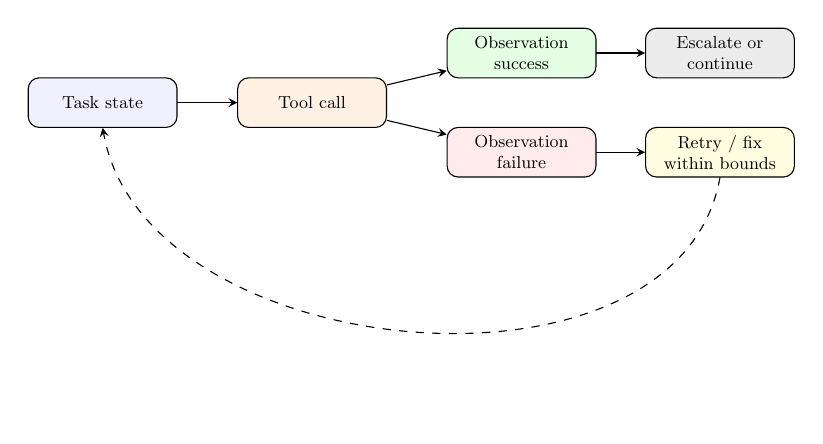
\begin{tikzpicture}[>=stealth,font=\small, scale=0.70, transform shape]
      \tikzset{box/.style={draw, rounded corners, minimum width=2.7cm, minimum height=0.9cm, align=center}}
      \node[box, fill=blue!6] (task) at (0,0) {Task state};
      \node[box, fill=orange!10] (tool) at (3.8,0) {Tool call};
      \node[box, fill=green!10] (ok) at (7.6,0.9) {Observation\\success};
      \node[box, fill=red!8] (fail) at (7.6,-0.9) {Observation\\failure};
      \node[box, fill=yellow!12] (retry) at (11.2,-0.9) {Retry / fix\\within bounds};
      \node[box, fill=gray!15] (human) at (11.2,0.9) {Escalate or\\continue};
      \draw[->] (task) -- (tool);
      \draw[->] (tool) -- (ok);
      \draw[->] (tool) -- (fail);
      \draw[->] (fail) -- (retry);
      \draw[->] (ok) -- (human);
      \draw[dashed,->] (retry.south) to[out=-100,in=-80] (task.south);
    \end{tikzpicture}
    \caption{Execution and recovery in an agentic workflow.}
  \end{figure}
\end{frame}

\begin{frame}{Significance of Recovery Logic}
  A robust workflow does not continue blindly after failure.

  It should:
  \begin{itemize}
    \item inspect the failure,
    \item attempt a bounded fix,
    \item escalate when uncertainty becomes too high.
  \end{itemize}

  In engineering, silent failure may be worse than explicit failure.
\end{frame}

\section{Skills, Tool Interfaces, and Orchestration}

\begin{frame}{Three Reusable Abstractions}
  As workflows become more capable, they are often organized around:
  \begin{itemize}
    \item \textbf{skills},
    \item \textbf{tool interfaces},
    \item \textbf{orchestration layers}.
  \end{itemize}

  These abstractions reduce improvisation and improve repeatability.
\end{frame}

\begin{frame}{Skills as Reusable Task Patterns}
  A skill is a reusable pattern for a class of work.

  Examples in engineering settings:
  \begin{itemize}
    \item manuscript review,
    \item note-to-slide conversion,
    \item codebase exploration,
    \item report validation,
    \item handoff generation.
  \end{itemize}

  Skills make systems more consistent by reducing ad hoc workflow invention.
\end{frame}

\begin{frame}{Tool Interfaces and Orchestration Layers}
  Tool interfaces define how external capabilities are called.

  Orchestration layers decide:
  \begin{itemize}
    \item which skill to invoke,
    \item which tool to call,
    \item whether to continue, retry, or escalate,
    \item how to preserve intermediate state,
    \item how to route work among specialized modules.
  \end{itemize}

  \begin{conceptbox}{System View}
    Frontier AI systems increasingly look like software architectures rather than just models.
  \end{conceptbox}
\end{frame}

\begin{frame}{Engineering Interpretation}
  Suppose an organization wants an AI assistant for bridge-inspection documentation.

  One skill may:
  \begin{itemize}
    \item summarize field notes,
    \item compare them against prior reports,
    \item search standards for relevant clauses.
  \end{itemize}

  The orchestration layer determines when to call each skill and when a human reviewer must intervene.
\end{frame}

\section{Automated Research Assistants}

\begin{frame}{Automated Research Assistants}
  A research-style agent is not a system that ``knows everything.''

  It is a system that can:
  \begin{itemize}
    \item search multiple sources,
    \item compare evidence,
    \item track unresolved questions,
    \item produce a structured synthesis.
  \end{itemize}

  This is one of the clearest real-world frontier applications of agentic AI.
\end{frame}

\begin{frame}{Verification-Driven Multi-Agent Orchestration}
  \begin{figure}
    \centering
    
\includegraphics[width=0.9\textwidth]{Topic17fig02.png}
    \caption{Verification-driven multi-agent orchestration.}
  \end{figure}
  \source{\href{https://arxiv.org/abs/2603.11445}{Zhang et al. (2026): Verified Multi-Agent Orchestration (VMAO)}}
\end{frame}

\begin{frame}{Significance of Verification-Driven Research Workflows}
  The VMAO diagram is pedagogically useful because it makes the verifier explicit.

  \begin{itemize}
    \item Planning is only the first step.
    \item Execution may happen in parallel.
    \item Verification checks completeness.
    \item Replanning occurs when gaps remain.
  \end{itemize}

  That is stronger than a generic loop because it makes quality control visible.
\end{frame}

\begin{frame}{Significance for Engineering Practice}
  Engineering work contains many research-like tasks:
  \begin{itemize}
    \item locate the controlling clause in a standard,
    \item inspect prior assumptions,
    \item compare guidance across documents,
    \item justify why one interpretation is safer than another.
  \end{itemize}

  A system that organizes those steps can save time, but it can also mislead if it hides uncertainty or provenance.
\end{frame}

\section{Human-in-the-Loop Engineering}

\begin{frame}{Human-in-the-Loop (HITL)}
  \begin{conceptbox}{Definition}
    A HITL system is one in which human review, intervention, or approval remains part of the operational workflow rather than being an afterthought.
  \end{conceptbox}

  In engineering, HITL is often a design requirement because the consequences of error can be physical, legal, financial, or ethical.
\end{frame}

\begin{frame}{Where Humans Sit in the Loop}
  Depending on the task, the human may:
  \begin{itemize}
    \item specify goals and constraints,
    \item approve access to tools,
    \item review intermediate evidence,
    \item validate the final result,
    \item audit the workflow after completion.
  \end{itemize}

  Different placements imply different risk tolerances.
\end{frame}

\begin{frame}{A Human-in-the-Loop Control Pattern}
  \begin{figure}
    \centering
    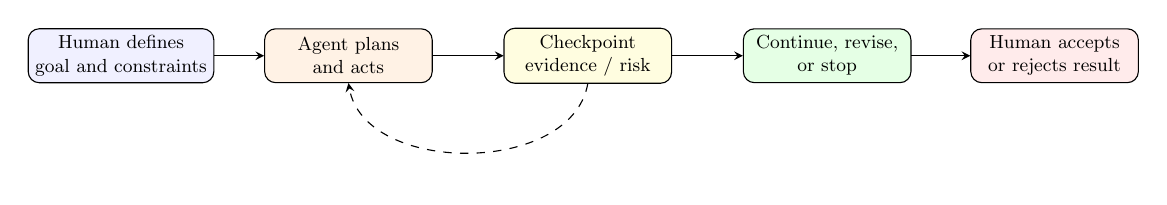
\begin{tikzpicture}[>=stealth,font=\small, scale=0.76, transform shape]
      \tikzset{box/.style={draw, rounded corners, minimum width=2.8cm, minimum height=0.9cm, align=center}}
      \node[box, fill=blue!6] (goal) at (0,0) {Human defines\\goal and constraints};
      \node[box, fill=orange!10] (agent) at (3.8,0) {Agent plans\\and acts};
      \node[box, fill=yellow!12] (checkpoint) at (7.8,0) {Checkpoint\\evidence / risk};
      \node[box, fill=green!10] (revise) at (11.8,0) {Continue, revise,\\or stop};
      \node[box, fill=red!8] (final) at (15.6,0) {Human accepts\\or rejects result};
      \draw[->] (goal) -- (agent);
      \draw[->] (agent) -- (checkpoint);
      \draw[->] (checkpoint) -- (revise);
      \draw[->] (revise) -- (final);
      \draw[dashed,->] (checkpoint.south) to[out=-100,in=-80] (agent.south);
    \end{tikzpicture}
    \caption{A HITL control pattern for agentic systems.}
  \end{figure}
\end{frame}

\begin{frame}{HITL as a Design Choice}
  If the human only sees the final polished answer, the loop may be too weak to matter.

  Good HITL design requires exposing:
  \begin{itemize}
    \item intermediate evidence,
    \item constraints,
    \item uncertainty,
    \item provenance,
    \item decision points.
  \end{itemize}

  The point is operational judgment, not ceremonial approval.
\end{frame}

\section{Failure Modes of Agentic AI}

\begin{frame}{Why Multi-Step Systems Fail Differently}
  Agentic systems inherit ordinary LLM weaknesses, but they also amplify them through multi-step behavior.

  Key failure modes include:
  \begin{itemize}
    \item compounding error,
    \item tool misuse,
    \item poor escalation behavior,
    \item goal drift.
  \end{itemize}
\end{frame}

\begin{frame}{Compounding Error and Tool Misuse}
  A wrong retrieval, wrong unit, or wrong file choice can contaminate later steps.

  Tool misuse adds more risk:
  \begin{itemize}
    \item wrong tool selected,
    \item wrong parameters passed,
    \item wrong output interpreted as valid.
  \end{itemize}

  Multi-step systems can therefore create longer chains of plausible but unsound behavior.
\end{frame}

\begin{frame}{Escalation Failure and Goal Drift}
  A system may:
  \begin{itemize}
    \item escalate too often and become useless,
    \item escalate too rarely and become reckless,
    \item drift toward local completion instead of the real engineering goal.
  \end{itemize}

  \begin{warningbox}{Important Caution}
    Multi-step capability does not automatically create deeper understanding. It can create longer chains of confident error.
  \end{warningbox}
\end{frame}

\section{Trust, Accountability, and Governance}

\begin{frame}{From Capability to Governance}
  As systems become more agentic, the question shifts from capability to governance.

  Key questions become:
  \begin{itemize}
    \item who approved the actions,
    \item what evidence was used,
    \item what logs exist,
    \item who is responsible when the system fails,
    \item what should never happen without human review.
  \end{itemize}
\end{frame}

\begin{frame}{Auditability and Traceability}
  Engineering culture already values documentation and checkability.

  An engineering agent should leave behind:
  \begin{itemize}
    \item its plan,
    \item actions,
    \item tool outputs,
    \item retrieved evidence,
    \item unresolved uncertainties.
  \end{itemize}

  That is how humans reconstruct whether a conclusion deserves trust.
\end{frame}

\begin{frame}{Responsibility Cannot Be Delegated}
  Accountability for an engineering decision cannot simply be assigned to the model.

  \begin{conceptbox}{Governance Principle}
    As systems gain longer horizons, tool access, and partial autonomy, the burden of auditability and explicit responsibility increases rather than decreases.
  \end{conceptbox}
\end{frame}

\section{Representative Agentic Systems in Practice}

\begin{frame}{Representative Systems in Practice}
  Before concluding, it helps to name systems that make agentic patterns concrete.

  Three useful categories are:
  \begin{itemize}
    \item web-navigation and research agents,
    \item software-engineering agents,
    \item frameworks and cognitive architectures.
  \end{itemize}
\end{frame}

\begin{frame}{Web-Navigation and Research Agents}
  Examples include:
  \begin{itemize}
    \item \textbf{WebGPT} — browser-based search and cited answers,
    \item automated research assistants — compare sources, track gaps, synthesize,
    \item verification-driven orchestration frameworks such as VMAO.
  \end{itemize}

  \source{\href{https://openai.com/research/webgpt}{OpenAI: WebGPT} \;|\; \href{https://arxiv.org/abs/2603.11445}{Zhang et al. (2026): VMAO}}
\end{frame}

\begin{frame}{Software Engineering Agents}
  Agentic behavior is also visible in systems such as:
  \begin{itemize}
    \item GPT Engineer,
    \item MetaGPT,
    \item newer coding agents that inspect repositories, propose edits, run checks, and continue over many steps.
  \end{itemize}

  Software engineering is pedagogically useful because tool calls, retries, and verification are often visible in the workflow.
\end{frame}

\begin{frame}{Frameworks and Architectures}
  At the framework level, students should recognize examples such as:
  \begin{itemize}
    \item LangChain-style agents,
    \item Toolformer-style tool-using language models,
    \item Soar-like architecture-level theories of intelligent behavior.
  \end{itemize}

  \begin{conceptbox}{Practical Takeaway}
    Agentic AI is not one product category. It is a family of workflow designs that combine planning, tools, state, and review in different proportions.
  \end{conceptbox}
\end{frame}

\section{Conclusion and Transition}

\begin{frame}{Design Principles for Engineering Agentic Systems}
  A practical summary:
  \begin{enumerate}
    \item use bounded autonomy,
    \item preserve evidence,
    \item escalate intentionally,
    \item design for recovery,
    \item log the process,
    \item keep the human decision where the risk is.
  \end{enumerate}
\end{frame}

\begin{frame}{Putting the Pieces Together}
  The course progression now looks like this:
  \begin{enumerate}
    \item Topic 15: language, retrieval, and evidence,
    \item Topic 16: usable systems built from prompts, retrieval, and tools,
    \item Topic 17: agentic workflows that plan, act, maintain state, recover, and escalate.
  \end{enumerate}

  The lesson is not to rush toward full autonomy. It is to decide how much agency is appropriate for which task.
\end{frame}

\begin{frame}{Reaching Less-Charted Waters}
  At this point in the course, both students and instructor are reaching less-charted waters.

  AI seems to be advancing in at least two directions:
  \begin{itemize}
    \item stronger foundation models, with new attention, memory, and possibly world-model-like paradigms,
    \item broader vertical applications, where many unmet needs may be accelerated by HITL workflows.
  \end{itemize}
\end{frame}

\begin{frame}{What Has Not Changed}
  Agentic systems can accelerate classical workflows, but many problems remain unresolved.

  \begin{warningbox}{Realistic Interpretation}
    AI, at least before speculative ASI, primarily amplifies human intentions, institutions, and incentives rather than creating new purposes of its own.
  \end{warningbox}

  This is not unusual; many revolutionary technologies have changed human activity through both leverage and disruption.
\end{frame}

\begin{frame}{From Topic 17 to Topic 18}
  Topic 18 will take a broader, more speculative but still fact-based view of the future discussion around AI:
  \begin{itemize}
    \item neural-symbolic systems beyond current agentic workflows,
    \item world models,
    \item ASI,
    \item embedded intelligence.
  \end{itemize}

  We will ask whether we even understand how to create genuinely embodied intelligence before speaking confidently about AI that broadly surpasses humans.
\end{frame}

\begin{frame}{Final Message}
  \begin{conceptbox}{Personal Engineering Slogan}
    Regardless of the paradigm, engineers stay above AI. We design it, constrain it, audit it, and remain responsible for how it enters the world.
  \end{conceptbox}
\end{frame}

\end{document}
